\سؤال{}

\textbf{ فرض کنید بعد از موضوع کرونا و ماجراهایش در کشور ما هم مجوز داروخانه صادر شده است. لذا دانشجویان کلاس مهندسی نرم‌افزار هم به این فکر افتادند که چنین نرم‌افزاری ایچاد نمایند. این نرم‌افزار نسخه تحت وب و اپلیکیشن خواهد داشت. نیازمندی‌های این سیستم را با روش‌های مختلفی که در فصل‌های مربوط به نیازمندی‌ها آموخته‌اید استخراج کرده و مستند کنید.}
\newline
با توجه به این که این سوال به صورت خیلی کلی طرح شده است، فرضیات مربوط به این سوال و سوال بعدی را در این قسمت نوشته و توضیح خواهم داد و نمودارها و نیازمندی‌ها با لحاظ این فرضیات نوشته و کشیده خواهند شد. \footnote{از آن‌جایی که کشیدن مدل‌های تحلیلی پیچیده در زمان امتحان امکان‌پذیر نیست، تلاش شده است تا حد امکان ساده و کاربردی پیاده‌سازی شوند.}

\begin{itemize}
	\item \textbf{نیازمندی‌ها\footnote{requirements} و موارد کاربرد\footnote{use-case}}
	
یک نرم‌افزار تحت وب و اپلیکیشن برای داروخانه طراحی می‌شود که در آن:
	\begin{enumerate}
		\item
		بیماران می‌توانند در سامانه ثبت‌نام کنند.
		\item 
		بیماران باید بتوانند وارد سامانه شوند.
		\item 
		متصدیان داروخانه باید بتوانند وارد سامانه شوند.
		\item 
		متصدیان داروخانه امکان اضافه کردن داروی جدید را دارند.
		\item 
		دارو شامل جزيیاتی مانند نام عمومی دارو، نام علمی دارو، نحوه‌مصرف، شکل و... هستند. این اطلاعات باید قابل مشاهده باشند.
		\item بیماران می‌توانند برگه‌های دفترچه بیمه و مربوط به داروهای خود را آپلود کنند.
		\item 
		متصدیان داروخانه برگه‌های دفترچه بیماران را بررسی می‌کنند.
		\item 
		امکان خرید آنلاین داروهای آزاد وجود دارد.

		\item 
		امکان جست‌وجو در لیست داروها باید پیاده‌سازی شود.
		\item 
		کاربران باید بتوانند از سیستم خارج شوند.

	\end{enumerate}

در بخش تحلیل نمودار‌های زیادی وجود دارند که می‌توان آن‌ها را رسم کرد و باعث ارتباط بهتر با مشتری می‌شود. در واقع در بخش فنی تنها در محدوده قلمرو مسئله\footnote{problem domain} هستیم و کاری به جزئیات فنی مانند پایگاه‌داده و ... نداریم. 

برخی نمودارهایی که در این بخش می‌توان رسم کرد عبارتند از: 

\begin{itemize}
	\item نمودار مورد کاربرد
	\item نمودار \lr{CRC}\footnote{در این نمودار رابطه‌ی بین مسئولیت‌ها و کلاس‌ها و نحوه‌ی همکاری آن‌ها نمایش داده می‌شود. منظور از}
	\item نمودار کلاس‌ها (بدون جزئیات فنی)
	\item و...
\end{itemize}
\item \textbf{نمودار مورد کاربرد}

در این نمودار ارتباط عوامل خارجی که به آن‌ها کنش‌گر\footnote{actor} گفته می‌شود با موارد کاربرد نمایش داده شده است. موارد کاربرد حتما باید خاصیت \lr{atomic} داشته باشند؛ به این معنی که قابل شکسته شدن به مورد کاربرد‌های کوچک‌تر نباشند. 


	\begin{figure}
		\begin{center}
			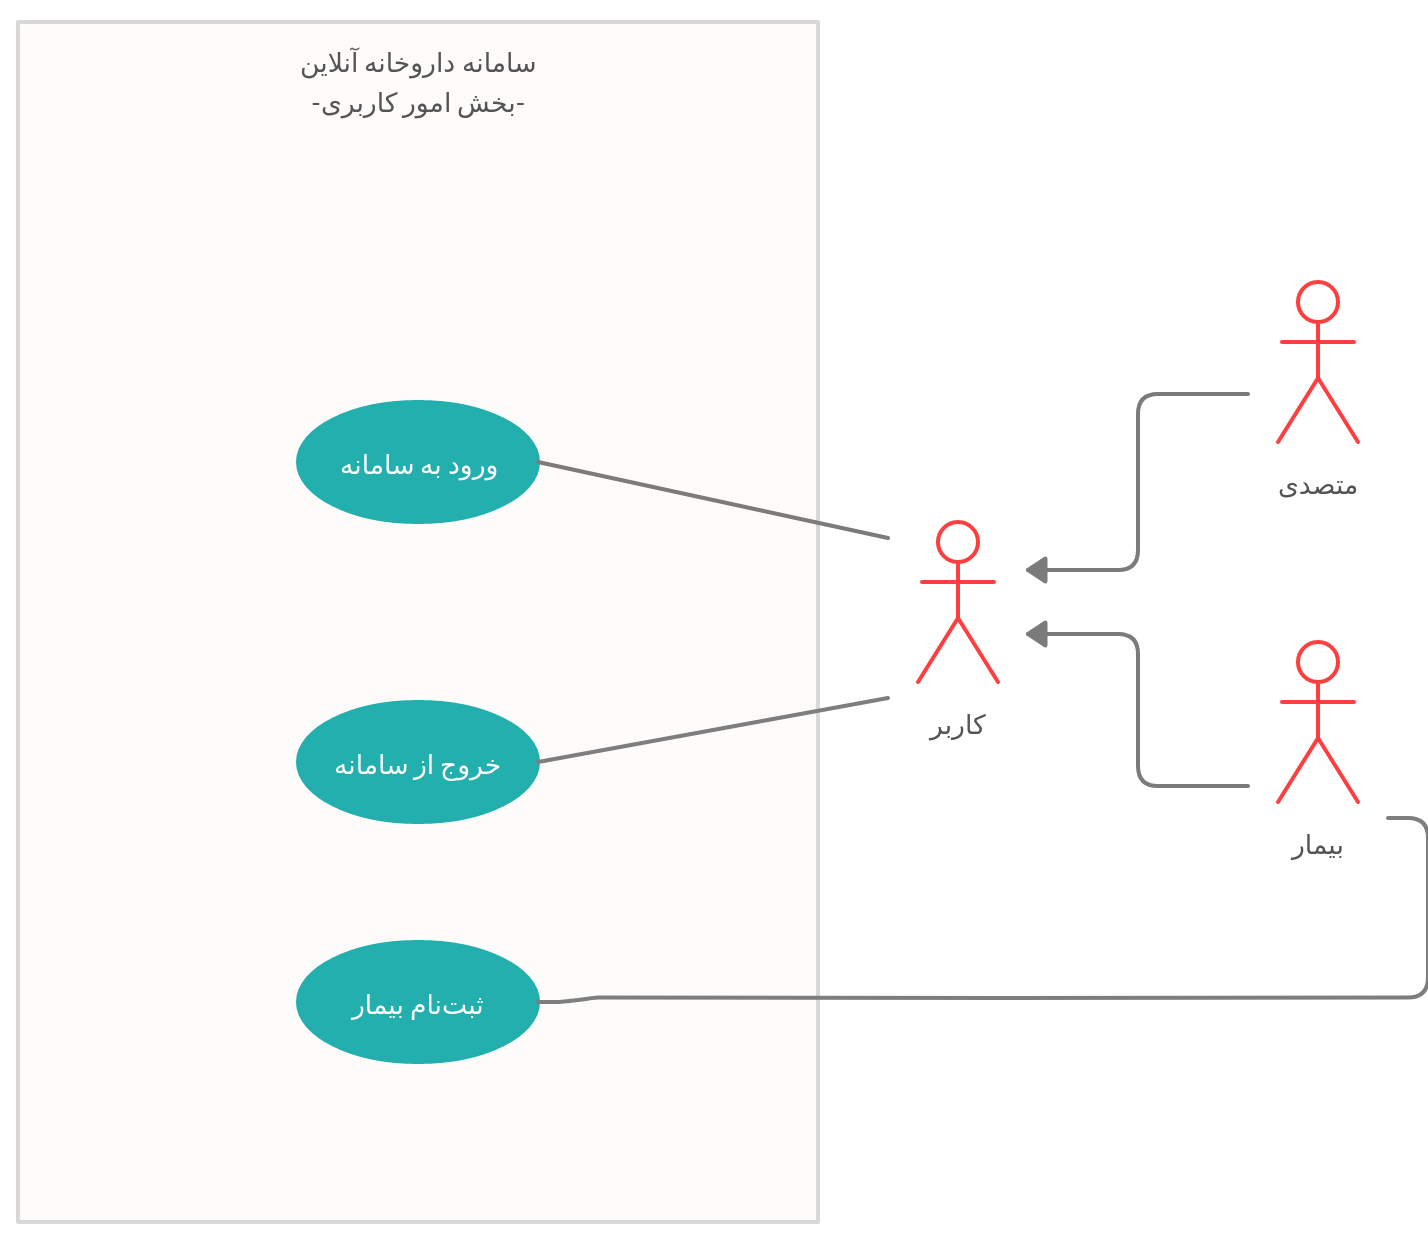
\includegraphics[scale=0.3]{./7-1.png}
			\caption{نمودار مورد کاربرد بخش امور کاربری}
		\end{center}
	\end{figure}
	\begin{figure}
		\begin{center}
			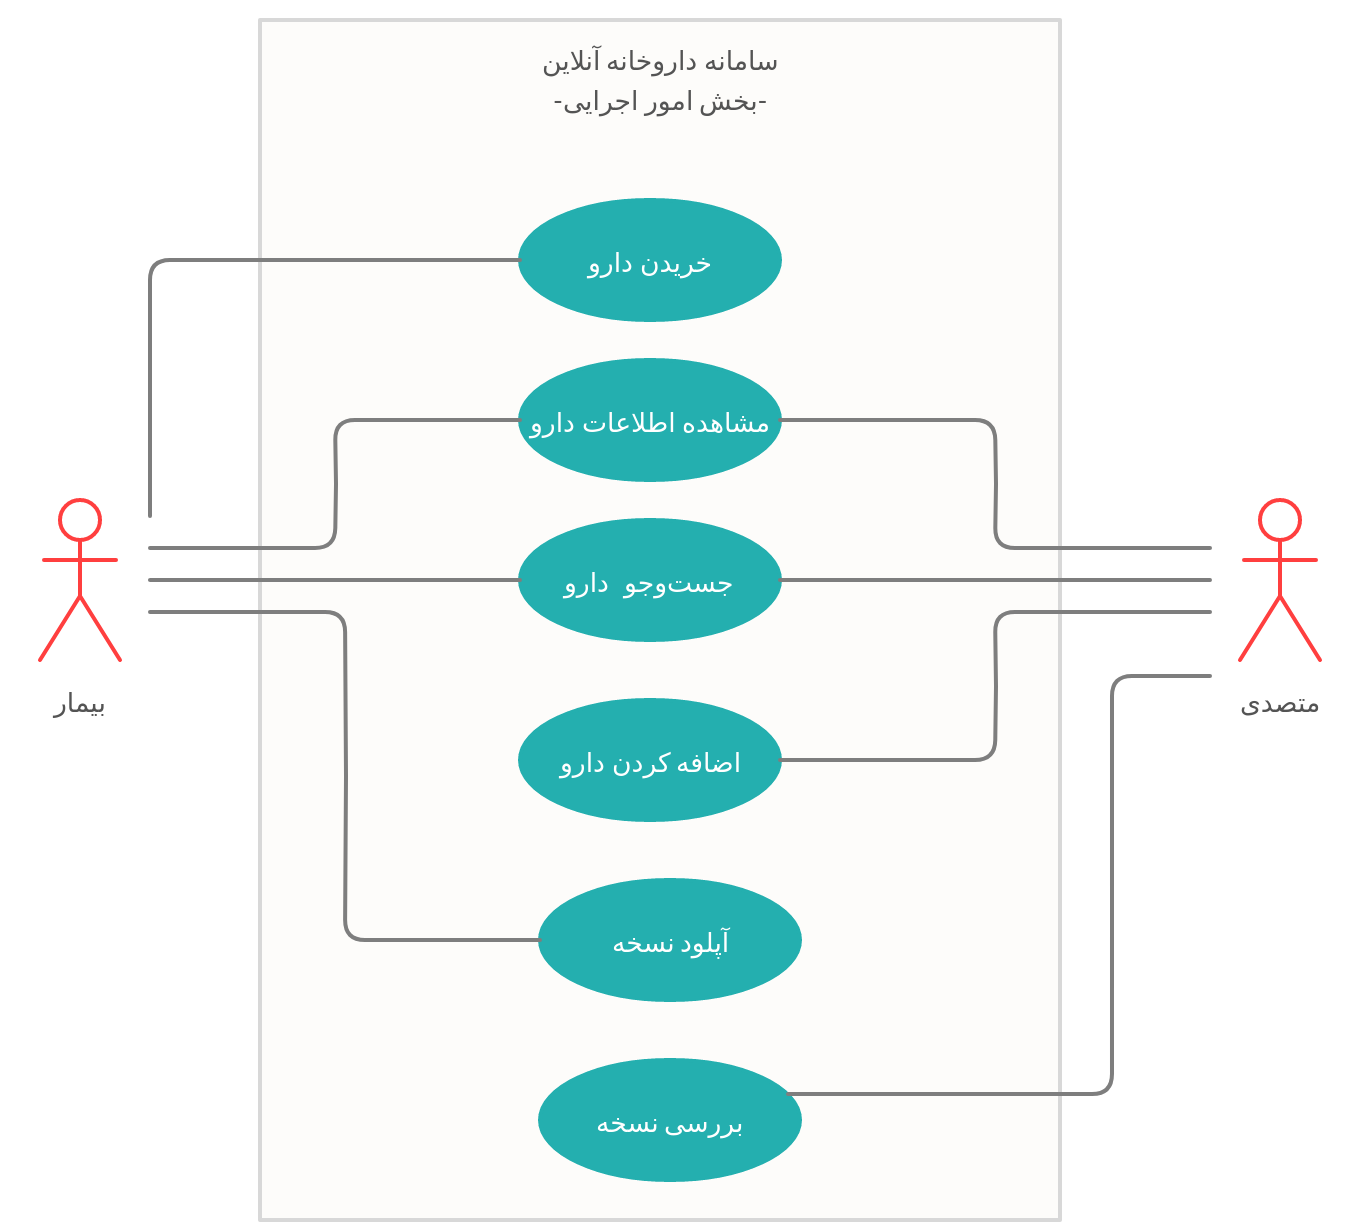
\includegraphics[scale=0.3]{./7-2.png}
			\caption{نمودار مورد کاربرد بخش امور اجرایی}
		\end{center}
	\end{figure}
\end{itemize}
